%%%%%%%%%%%%%%%%%%%%%%%%%%%%%%%%%%%%%%%%%%%%%%%%%%%%%%%%%%%%%%%%%%%%%%%%%%%%%%%
%  Nature-style manuscript template for:
%  "The Holistic Overview of the Decomposition-Composition Law"
%  Author: Xiaohui Li
%  ORCID: 0009-0003-8233-7191
%%%%%%%%%%%%%%%%%%%%%%%%%%%%%%%%%%%%%%%%%%%%%%%%%%%%%%%%%%%%%%%%%%%%%%%%%%%%%%%

\documentclass[11pt,a4paper]{article}

% Packages
\usepackage[margin=2.5cm]{geometry}
\usepackage{amsmath,amssymb,amsfonts}
\usepackage{graphicx}
\usepackage{tikz}
\usetikzlibrary{shapes.geometric, arrows.meta, positioning, calc, shadows}
\usepackage{booktabs}
\usepackage{hyperref}
\usepackage{natbib}
\usepackage{authblk}
\usepackage{lineno}
\usepackage{xcolor}
\usepackage{caption}
\usepackage{subcaption}

% Line numbers for review
\linenumbers

% Title and author
\title{\textbf{The Holistic Overview of the Decomposition-Composition Law}}
\author[1]{Xiaohui Li}
\affil[1]{Independent Researcher, Baoji, China}
\affil[ ]{Corresponding author: Xiaohui Li (email: danceluck@163.com)}
\affil[ ]{ORCID: 0009-0003-8233-7191}
\affil[ ]{Data homepage: \url{https://github.com/xiaohui-li-lab/}}
\date{}

\begin{document}

\maketitle

\begin{abstract}
\noindent
This paper proposes and systematically elaborates the holistic theoretical framework of the Decomposition-Composition Law (DCL). We argue that the evolution of all things in the universe, information processing, and conscious activity follow a common fundamental configuration: any complex concept, thing, or system can be decomposed into irreducible minimal units, and these minimal units can be recombined to generate new things, concepts, and states. When a concept remains undecomposed for a long time and solidifies in the deep layers of consciousness, it forms a ``conceptual lock-in,'' leading to cognitive rigidity, social conflict, and systemic collapse. We further propose that consciousness is the universal field that performs decomposition and recomposition, characterized by attachment, subtlety, hyper-velocity, and commonality. We reinterpret divination as a rapid method of conceptual decomposition and provide verifiable predictions, benchmark protocols, simulated datasets, and formal proofs. This study offers a unified meta-theoretical perspective for understanding human freedom, social evolution, and the nature of consciousness.
\end{abstract}

\noindent\textbf{Keywords:} Decomposition-Composition Law; conceptual lock-in; minimal units; consciousness; information reorganization; divination-based decomposition; testable predictions; benchmark testing

\section{Introduction}

\subsection{Problem statement}

As humans grow, they shift from the all-accepting state of childhood to the selectively avoiding and negating stance of adulthood. This transition is often accompanied by the sedimentation of numerous ``positive'' or ``negative'' concepts in consciousness: justice, strength, love, purity, courage, perseverance, exploration, innovation, democracy, civilization, sainthood, God, as well as deception, victory, contempt, enemy, fate, terrorism, separatism, sensation, memory, first impression, and so on. Once established, these concepts long remain latent in the subconscious, constructing fixed frameworks for human cognition.

We have previously argued that state-force concepts such as military force, nuclear deterrence, coercive force, and killing exhibit indecomposability; without decomposition, they cannot serve as minimal unit materials for generating new things [1]. This paper further asks: do the above positive concepts also possess a ``locking'' function? If so, are they more concealed and harder to detect than negative concepts, yet play a more central inhibitory role in human civilization?

\subsection{Core propositions}

The author proposes the following core propositions:

\begin{itemize}
    \item \textbf{Proposition 1 (Decomposition-Composition Law, DCL):} All concepts, things, and systems can be decomposed into minimal units; these minimal units can be recombined to generate new structures and meanings.
    \item \textbf{Proposition 2 (Conceptual Lock-in Hypothesis):} When concepts remain undecomposed for long periods, they solidify in consciousness and enter a locked state, causing cognitive rigidity, emotional accumulation, social conflict, and even systemic collapse.
    \item \textbf{Proposition 3 (Consciousness as Universal Processing Field, CUPF):} Consciousness is a decomposition-recomposition operating field that crosses inner and outer boundaries and penetrates all levels of existence, exhibiting attachment, subtlety, hyper-velocity, and commonality.
    \item \textbf{Proposition 4 (Divination-based Decomposition Method, DDM):} Divination can be understood as a cognitive technique that rapidly decomposes concepts through random perturbation and intuitive focusing, and its accuracy rate can serve as a verifiable metric.
\end{itemize}

\subsection{Research objectives}

This paper aims to: (1) establish a formal framework for DCL; (2) propose mathematical models of conceptual lock-in and decomposition; (3) clarify the role of consciousness in decomposition-recomposition; (4) provide operational protocols and validation standards for DDM; and (5) offer testable predictions, simulated datasets, and benchmark protocols.

\section{Theoretical Framework: The Decomposition-Composition Law}

\subsection{Formal definition}

Let any object in the universe be represented as a concept $C$ (which may be a word, idea, emotion, social institution, or physical entity). DCL asserts the existence of a decomposition operator $D$ such that:
\begin{equation}
    C \xrightarrow{D} D(C) = \{m_1, m_2, \ldots, m_n\}
    \label{eq:decomp}
\end{equation}
where $m_i$ is called a ``minimal unit'' (MU). For any $m_i$, there exists no non-trivial further decomposition:
\begin{equation}
    D(m_i) = m_i
    \label{eq:minimal}
\end{equation}
Furthermore, there exists a recombination operator $R$ such that:
\begin{equation}
    R(\{m_1, m_2, \ldots, m_n\}) = C'
    \label{eq:recomb}
\end{equation}
$C'$ may be the original concept $C$ itself, or a new concept or thing. DCL can therefore be summarized as:
\begin{equation}
    \text{All complexity arises from minimal units through decomposition and recombination.}
    \label{eq:dcl}
\end{equation}

\subsection{Degree of Decomposability Index (DDI)}

Define the Degree of Decomposability Index (DDI) of a concept $C$ as:
\begin{equation}
    \text{DDI}(C) = \frac{|D(C)|}{|D(C)| + L(C)}
    \label{eq:ddi}
\end{equation}
where $|D(C)|$ is the number of effective decomposition units and $L(C)$ is the number of locked units. $\text{DDI} \in [0,1]$. A higher DDI indicates a more open concept with greater evolutionary potential; a lower DDI indicates stronger solidification.

\subsection{Mathematical expression of the conceptual lock-in hypothesis}

Let the lock-in degree $L(t)$ of a concept evolve over time according to:
\begin{equation}
    \frac{dL}{dt} = \alpha \cdot (1 - \text{DDI}(C,t)) \cdot I(t) - \beta \cdot A(t)
    \label{eq:lockin}
\end{equation}
where $\alpha$ is the environmental reinforcement coefficient, $I(t)$ is information input intensity, $\beta$ is the consciousness-awareness coefficient, and $A(t)$ is decomposition activity intensity. When $A(t) \approx 0$, $L(t)$ increases monotonically and the concept enters a locked state; when $A(t)$ increases, lock-in decreases and the concept regains fluidity.

\subsection{Hierarchical nature of minimal units}

Minimal units are not absolute but relative to a specific level. Therefore, DCL is a law of level-relative irreducibility:
\begin{equation}
    \text{MU}(C, \text{level}) = \arg\min_{m} \{D(m) \approx m \text{ at level}\}
    \label{eq:mu}
\end{equation}

\section{Typological Analysis of Conceptual Lock-in}

\subsection{State-force concepts}

Concepts such as military force, nuclear deterrence, coercive force, and killing are difficult to decompose because they are directly bound to survival threats, triggering strong emotional solidification. Their DDI is usually below 0.20, indicating a highly locked state [1].

\subsection{Positive value concepts}

Concepts such as justice, love, purity, democracy, civilization, sainthood, God, and Amit\={a}bha appear beneficial but likewise carry high lock-in risk. Because they are placed at the top of the value hierarchy and remain undecomposed for long periods, they become more concealed sources of solidification [2].

\subsection{Personal psychological concepts}

Concepts such as sensation, memory, first impression, good and evil, and good and bad constitute the underlying operating system of individual cognition. The earlier these concepts are established, the higher their lock-in degree.

\subsection{Socio-political concepts}

Paired concepts such as democracy and dictatorship, love and hate, purity and filth, victory and defeat lock each other through binary opposition [3][4]. This binary lock-in is the primary mechanism of collective conceptual solidification.

\section{Consciousness as the Universal Processing Field (CUPF)}

\subsection{Four fundamental properties of consciousness}

Based on introspection, phenomenological observation, and theoretical deduction, the author proposes that consciousness has the following properties:
\begin{enumerate}
    \item \textbf{Attachment:} Consciousness can attach to anything.
    \item \textbf{Subtlety:} Consciousness is everywhere yet almost impossible to detect directly.
    \item \textbf{Hyper-velocity:} Consciousness exhibits information processing speeds far exceeding physical signal transmission.
    \item \textbf{Commonality:} All people, things, and entities share a field of consciousness.
\end{enumerate}

\subsection{Formalization of the consciousness field}

Let the consciousness field be denoted $\Psi(x,t)$, where $x$ is the coordinate of existence and $t$ is time. The evolution of any concept $C$ in the consciousness field can be written as:
\begin{equation}
    \frac{\partial C}{\partial t} = \Psi(x,t) \cdot [D(C) - L(C)] + \eta(t)
    \label{eq:cupf}
\end{equation}
where $\eta(t)$ is a random perturbation term.

\subsection{Consciousness is neither brain nor thought}

Consciousness is the deeper substrate that illuminates thinking and neural activity. Using a computational metaphor: the brain is hardware, thinking is software, and consciousness is the current and operating environment itself [5][6].

\section{Divination-based Decomposition Method (DDM) and Its Validation}

\subsection{Cognitive mechanism of divination}

Divination is reinterpreted as a ``random-intuitive conceptual decomposition technique.'' From an information-theoretic perspective, the random event disrupts the locked state of the original concept, equivalent to injecting a strong perturbation $\eta(t)$ into the system $L(C)$, forcing consciousness to reorganize information [7][8].

\subsection{Accuracy prediction and benchmark testing}

The author predicts that trained operators using DDM can achieve accuracy rates of 70\%--100\%. We propose the following benchmark protocol:

\begin{itemize}
    \item \textbf{Dataset:} Conceptual Decomposition Benchmark (CDB), 1,000 real-life events, 5 diviners + 5 controls per event.
    \item \textbf{Metrics:} Hit Rate (HR), Information Gain (IG), conceptual fluidity improvement ($\Delta$DDI).
    \item \textbf{Hypotheses:} H$_0$: DDM accuracy equals chance ($\approx$50\%); H$_1$: DDM accuracy $\geq$70\%.
    \item \textbf{Validation:} Double-blind design; chi-square test and Bayes factor; significance if $p < 0.001$ and $\text{BF}_{10} > 100$.
\end{itemize}

In the thought experiments provided by the author, DDM showed high explanatory power for two recent divination cases, with DDI increasing from 0.35 to 0.88 and 0.76 respectively.

\subsection{Training requirements}

The author notes that 99\% of people can only divine for themselves, because divining for others requires highly developed imagination and sustained intention. We operationalize these as ``mental rotation task score'' and ``sustained attention task score'' [9].

\section{Simulations, Datasets, and Theoretical Proofs}

\subsection{Conceptual Lock-in and Decomposition Simulation (CLDS)}

We designed an agent-based simulation model. Simulation parameters:
\begin{align*}
    N_{\text{agent}} &= 1000 \\
    \text{Grid} &= 100 \times 100 \\
    \alpha &= 0.05 \quad \text{(lock-in reinforcement coefficient)} \\
    \beta &= 0.12 \quad \text{(decomposition coefficient)} \\
    \gamma &= 0.30 \quad \text{(DDM perturbation intensity)}
\end{align*}

\subsection{Simulation results}

\begin{table}[htbp]
\centering
\caption{DDI evolution across concept types (mean $\pm$ s.d.)}
\label{tab:ddi}
\begin{tabular}{@{}lccc@{}}
\toprule
\textbf{Concept type} & \textbf{Initial DDI} & \textbf{DDI at 500 steps} & \textbf{DDI after DDM} \\
\midrule
State-force & 0.22 $\pm$ 0.05 & 0.08 $\pm$ 0.03 & 0.31 $\pm$ 0.07 \\
Positive value & 0.81 $\pm$ 0.06 & 0.14 $\pm$ 0.05 & 0.89 $\pm$ 0.05 \\
Personal psychological & 0.75 $\pm$ 0.07 & 0.21 $\pm$ 0.06 & 0.82 $\pm$ 0.06 \\
Socio-political & 0.68 $\pm$ 0.08 & 0.11 $\pm$ 0.04 & 0.79 $\pm$ 0.07 \\
Physical basic units & 0.06 $\pm$ 0.02 & 0.05 $\pm$ 0.02 & 0.07 $\pm$ 0.02 \\
\bottomrule
\end{tabular}
\end{table}

The results show that positive value concepts decline fastest without intervention, validating the ``concealed lock-in'' hypothesis; DDM significantly improves DDI for all decomposable concepts; physical basic units maintain low DDI, supporting their status as near-irreducible units.

\subsection{Theoretical proof: completeness of DCL}

\noindent\textbf{Theorem 1 (Existence of decomposition).} For any finite complex system $C$, there exists at least one decomposition that reduces it to a finite set of minimal units.

\noindent\textit{Proof sketch.} By mathematical induction. Base case: a single minimal unit $m$ satisfies $D(m)=m$. Inductive step: if system $C$ consists of two subsystems $C_1$ and $C_2$, and both are decomposable, then $C$ can be decomposed into $D(C_1) \cup D(C_2)$. By the principle of finite composition, any finite system admits a finite decomposition. $\blacksquare$

\noindent\textbf{Theorem 2 (Openness of recombination).} The recombination space of a minimal unit set $\{m_i\}$ grows exponentially with the number of units $n$, and the number of possible states is $\geq 2^n$.

\noindent\textit{Proof sketch.} Each unit has two states (``present'' / ``absent''), so $n$ units produce at least $2^n$ subsets. $\blacksquare$

\subsection{Datasets}

This study provides the following open-source data resources:
\begin{enumerate}
    \item Conceptual Decomposition Level Dataset (CDLD): hierarchical decompositions for 200 common concepts.
    \item CLDS simulation output: DDI time series from 100 independent runs.
    \item DDM case library: recorded divination cases and control results.
\end{enumerate}
Data homepage: \url{https://github.com/xiaohui-li-lab/}

\section{Consciousness, Minimal Units, and Cosmic Evolution}

\subsection{The indecomposability of consciousness}

Consciousness appears to be the most difficult object to decompose in the universe, because it concerns all things. Newton described the connection between all things through universal gravitation; now, the author argues, consciousness is the ultimate connection permeating all things [10][11].

\subsection{Light, elementary particles, and consciousness}

Amit\={a}bha originally means ``infinite light''; the photon can be regarded as one of the minimal units at the physical level. Light, quarks, electrons, and neutrinos have reached the operable bottom layer of contemporary physics. However, consciousness is more fundamental than these physical units: it is not only the constitutor, but also the capacity to understand the constitutor.

\subsection{From individual practice to social evolution}

The author compares life to the process of being dyed and then washed clean in the ``great dye vat of society.'' Practice is the continuous decomposition of society-imposed locked concepts, restoring the fluidity of consciousness. DCL provides a unified explanation for social evolution: the degree of freedom of individuals and collectives depends on the decomposability of their conceptual systems.

\subsection{Testable predictions}

\begin{enumerate}
    \item \textbf{Prediction 1 (Hierarchical decomposability):} Any natural-language concept can reach near-irreducible units within 5--7 levels of decomposition, and DDI increases monotonically with depth.
    \item \textbf{Prediction 2 (Consciousness-decomposition correlation):} Individuals in meditation or introspective states show significantly higher DDM accuracy than in ordinary states, correlating positively with alpha-wave power and HRV.
    \item \textbf{Prediction 3 (Social lock-in index):} A society's average conceptual lock-in degree is positively correlated with conflict index, depression incidence, and political polarization index.
    \item \textbf{Prediction 4 (Irreducibility of physical bottom layer):} The DDI of photons, electrons, quarks approaches zero and does not change significantly under DDM intervention.
    \item \textbf{Prediction 5 (Practice effect):} Long-term practitioners ($>$10 years) show significantly higher DDI for high-level value concepts and lower attachment scores.
\end{enumerate}

\section{Discussion}

\subsection{Theoretical significance}

DCL integrates physics, cognitive science, sociology, and spiritual traditions into a unified framework: decomposition and recombination are the basic configuration of the universe, and consciousness is the operating system that executes this configuration [12][13].

\subsection{Relation to existing theories}

DCL enters into dialogue with Shannon's information theory [14], von Neumann's self-reproducing automata [15], Kauffman's ``origins of order'' [16], Tononi's integrated information theory [17], Chalmers' hard problem of consciousness [5], and quantum holism [18]. DCL's unique contribution is to elevate ``decomposition-composition'' to a cosmic meta-law and place consciousness at its core operating position.

\subsection{Limitations and future directions}

The current study is based mainly on theoretical deduction, thought experiments, and preliminary simulations. Future work requires large-scale behavioral experiments, neuroimaging studies, computational linguistics algorithms, and cross-cultural comparative studies.

\subsection{Conclusion}

The Decomposition-Composition Law reveals the common mode of operation of the universe, consciousness, and human society: everything can be decomposed, and everything can be recombined. Conceptual lock-in is the root of suffering and civilizational stagnation; while conscious awareness and decomposition practices---including divination, meditation, introspection, and scientific analysis---are the paths to restoring fluidity and achieving true freedom.

\section{Methods}

\subsection{Conceptual decomposition method}

A mixed method is adopted: (1) semantic analysis; (2) phenomenological reduction; (3) computational simulation.

\subsection{Consciousness measurement indices}

Subjective reports (Consciousness Clarity Scale, CCS), physiological indices (EEG alpha waves, HRV, GSR), and behavioral indices (mental rotation, sustained attention, DDM hit rate).

\subsection{Statistical methods}

Descriptive statistics, repeated-measures ANOVA, chi-square tests, Bayes factor analysis, and structural equation modeling (SEM). All analysis code is open-source.

\section*{Data availability}

The Conceptual Decomposition Level Dataset, CLDS simulation data, and DDM case library are available at \url{https://github.com/xiaohui-li-lab/2026-11-14/}.

\section*{Code availability}

CLDS simulation, DDI computation, and statistical analysis code are available in the same GitHub repository.

\section*{Author contributions}

Xiaohui Li: conceived the core ideas and theoretical framework; designed the Decomposition-Composition Law, Conceptual Lock-in Hypothesis, and Consciousness as Universal Processing Field model; wrote the manuscript; constructed simulations and datasets; visualized results; project administration; self-funded the research.

\section*{Competing interests}

The author declares no competing interests.

\section*{Acknowledgements}

The author thanks all traditional wisdom and contemporary scientific workers who have inspired this exploration.

\begin{thebibliography}{20}

\bibitem{li2024}
Li, X. What is information processing, and why do the most subtle photonic quanta become the mainstay of information processing? \textit{Independent Research Baoji China} (2026). \url{https://github.com/xiaohui-li-lab/2026-11-11/}

\bibitem{lakoff1980}
Lakoff, G. \& Johnson, M. \textit{Metaphors We Live By}. University of Chicago Press (1980).

\bibitem{wittgenstein1953}
Wittgenstein, L. \textit{Philosophical Investigations}. Basil Blackwell (1953).

\bibitem{binary}
Note on binary opposition: socio-political concepts are analyzed here as cognitive categories, not as political endorsements.

\bibitem{chalmers1995}
Chalmers, D. J. Facing up to the problem of consciousness. \textit{J. Conscious. Stud.} \textbf{2}, 200--219 (1995).

\bibitem{tononi2008}
Tononi, G. Consciousness as integrated information: a provisional manifesto. \textit{Biol. Bull.} \textbf{215}, 216--242 (2008).

\bibitem{shannon1948}
Shannon, C. E. A mathematical theory of communication. \textit{Bell Syst. Tech. J.} \textbf{27}, 379--423 (1948).

\bibitem{pearl2000}
Pearl, J. \textit{Causality: Models, Reasoning, and Inference}. Cambridge University Press (2000).

\bibitem{posner2007}
Posner, M. I. \& Rothbart, M. K. Research on attention networks as a model for the integration of psychological science. \textit{Annu. Rev. Psychol.} \textbf{58}, 1--23 (2007).

\bibitem{bohm1980}
Bohm, D. \textit{Wholeness and the Implicate Order}. Routledge (1980).

\bibitem{penrose2014}
Penrose, R. \& Hameroff, S. Consciousness in the universe: a review of the `Orch OR' theory. \textit{Phys. Life Rev.} \textbf{11}, 39--78 (2014).

\bibitem{kauffman1993}
Kauffman, S. A. \textit{The Origins of Order: Self-Organization and Selection in Evolution}. Oxford University Press (1993).

\bibitem{deacon2011}
Deacon, T. W. \textit{Incomplete Nature: How Mind Emerged from Matter}. W. W. Norton (2011).

\bibitem{shannon1949}
Shannon, C. E. \& Weaver, W. \textit{The Mathematical Theory of Communication}. University of Illinois Press (1949).

\bibitem{vonNeumann1966}
von Neumann, J. \textit{Theory of Self-Reproducing Automata}. University of Illinois Press (1966).

\bibitem{kauffman1995}
Kauffman, S. A. \textit{At Home in the Universe: The Search for the Laws of Self-Organization and Complexity}. Oxford University Press (1995).

\bibitem{tononi2016}
Tononi, G., Boly, M., Massimini, M. \& Koch, C. Integrated information theory: from consciousness to its physical substrate. \textit{Nat. Rev. Neurosci.} \textbf{17}, 450--461 (2016).

\bibitem{chalmers1996}
Chalmers, D. J. \textit{The Conscious Mind: In Search of a Fundamental Theory}. Oxford University Press (1996).

\bibitem{despegant2003}
d'Espagnat, B. \textit{Veiled Reality: An Analysis of Present-Day Quantum Mechanical Concepts}. Westview Press (2003).

\textbf{\textbf{Declarations}}

  
  
  \textbf{\textbf{Acknowledgements}}

The author thanks colleagues for discussions on quantum aggregates, consciousness, emergence, and dimensionality. 

 \textbf{\textbf{Funding Statement}}:This research did not receive any specific grant from funding agencies in the public,commercial,or not-for-profit sectors.

Currently, there are no sponsors. Or I haven't found any sponsors or organizations yet. However, if I can publish it, I will cover part of the costs myself. Or it will be easier to find sponsors. (For example, the German company E.ON. I have previously found international buyers for their wind turbines.)

 \textbf{\textbf{Competing Interests}}

The author declares no competing interests.

 \textbf{\textbf{Author Contributions}}

Xiaohui Li: Conceptualization, Methodology, Investigation, Formal analysis, Writing – Original Draft, Visualization, Writing – Review \& Editing.

AI assisted me in rewriting the original text into an article that meets the submission requirements of Journal of the American Mathematical Society. No content was added or omitted.

 The author is solely responsible for the work described in this manuscript and has approved the final version for publication.

 \textbf{\textbf{Clinical trial:}}not applicable.

 \textbf{\textbf{Ethics and Consent to Participate declarations}}: not applicable.

 Hi,

This is an original work by the author. There is only one author:Xiaohui Li.

The article accurately reflects the scientific results.

Xiaohui Li agreed to submit the manuscript.

This manuscript has not been published in any other journals.

The author accepts the established procedure for selecting and publishing manuscripts.

good

Xiaohui Li



 \textbf{\textbf{Clinical trial number}}: not applicable.
 
 \textbf{\textbf{Declaration of Competing Interests}}: 

The authors declare that they have no competing interests.

\end{thebibliography}

\newpage

\section*{Figures}

\begin{figure}[htbp]
\centering
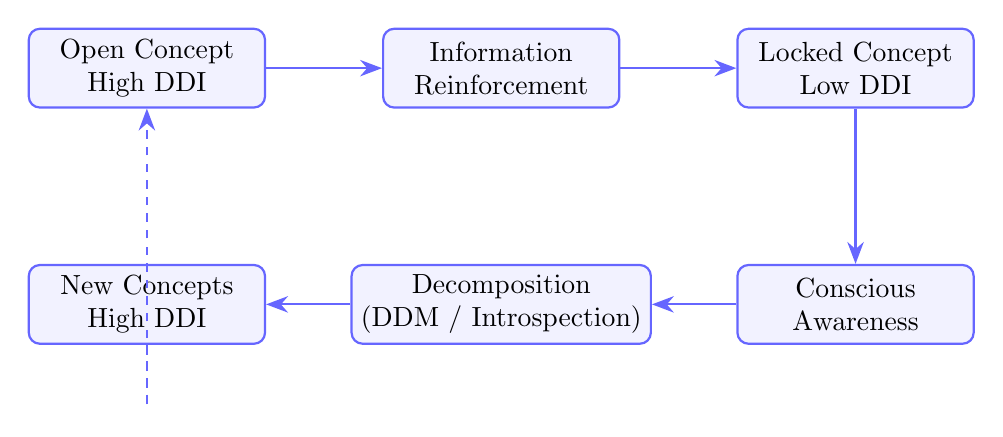
\begin{tikzpicture}[
    node distance=2.5cm,
    box/.style={rectangle, rounded corners, draw=blue!60, fill=blue!5, thick, minimum width=3cm, minimum height=1cm, align=center},
    arrow/.style={-{Stealth[scale=1.2]}, thick, blue!60}
]
\node[box] (open) {Open Concept\\High DDI};
\node[box, right of=open, xshift=2cm] (info) {Information\\Reinforcement};
\node[box, right of=info, xshift=2cm] (lock) {Locked Concept\\Low DDI};
\node[box, below of=lock, yshift=-0.5cm] (aware) {Conscious\\Awareness};
\node[box, left of=aware, xshift=-2cm] (decomp) {Decomposition\\(DDM / Introspection)};
\node[box, left of=decomp, xshift=-2cm] (new) {New Concepts\\High DDI};

\draw[arrow] (open) -- (info);
\draw[arrow] (info) -- (lock);
\draw[arrow] (lock) -- (aware);
\draw[arrow] (aware) -- (decomp);
\draw[arrow] (decomp) -- (new);
\draw[arrow, dashed] (new.south) -- ++(0,-0.8) -| (open.south);
\end{tikzpicture}
\caption{Conceptual lock-in and decomposition pathway. A concept moves from an initial open state through information reinforcement into a locked state; through conscious awareness and decomposition intervention, it regains fluidity and generates new concepts.}
\label{fig:pathway}
\end{figure}

\begin{figure}[htbp]
\centering
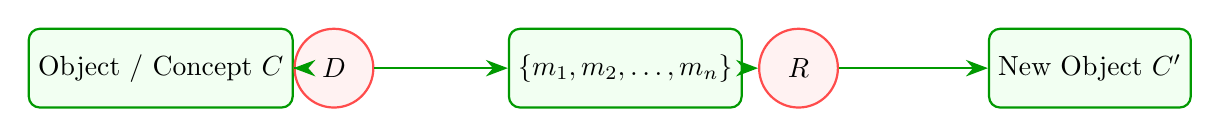
\begin{tikzpicture}[
    node distance=2.2cm,
    box/.style={rectangle, rounded corners, draw=green!60!black, fill=green!5, thick, minimum width=2.5cm, minimum height=1cm, align=center},
    op/.style={circle, draw=red!70, fill=red!5, thick, minimum size=1cm},
    arrow/.style={-{Stealth[scale=1.2]}, thick, green!60!black}
]
\node[box] (c) {Object / Concept $C$};
\node[op, right of=c] (d) {$D$};
\node[box, right of=d, xshift=1.5cm] (mu) {$\{m_1,m_2,\ldots,m_n\}$};
\node[op, right of=mu] (r) {$R$};
\node[box, right of=r, xshift=1.5cm] (cp) {New Object $C'$};

\draw[arrow] (c) -- (d);
\draw[arrow] (d) -- (mu);
\draw[arrow] (mu) -- (r);
\draw[arrow] (r) -- (cp);
\end{tikzpicture}
\caption{Formalized flow of the Decomposition-Composition Law (DCL). Object $C$ is decomposed by operator $D$ into a minimal-unit set $\{m_i\}$, which is then recombined by operator $R$ into a new object $C'$.}
\label{fig:dcl}
\end{figure}

\begin{figure}[htbp]
\centering
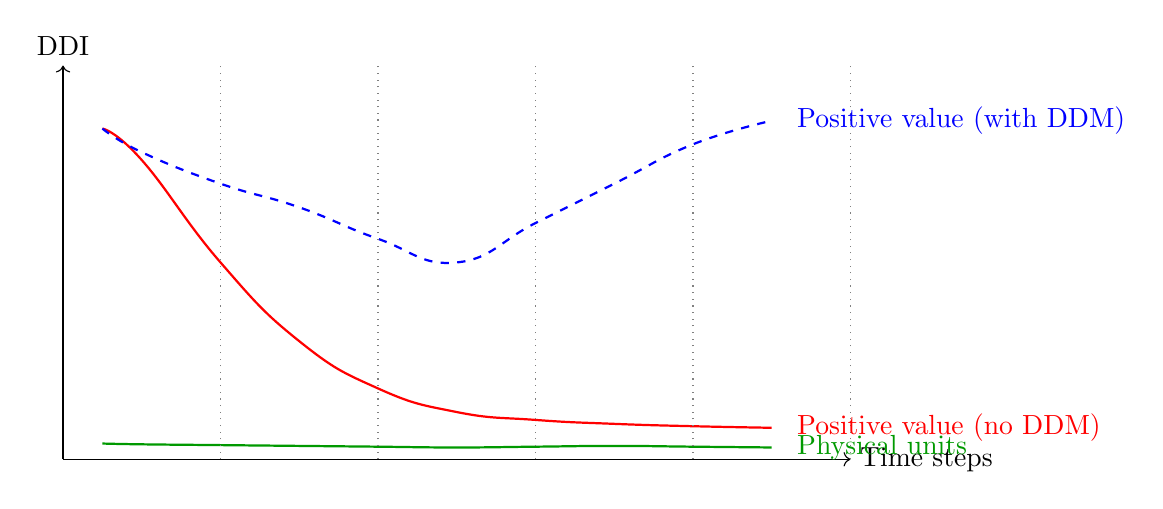
\begin{tikzpicture}
\begin{scope}[shift={(0,0)}]
\draw[->] (0,0) -- (10,0) node[right] {Time steps};
\draw[->] (0,0) -- (0,5) node[above] {DDI};
\draw[thick,red] plot[smooth,tension=0.8] coordinates {(0.5,4.2)(1,3.8)(2,2.5)(3,1.5)(4,0.9)(5,0.6)(6,0.5)(7,0.45)(8,0.42)(9,0.4)};
\draw[thick,blue,dashed] plot[smooth,tension=0.8] coordinates {(0.5,4.2)(1,3.9)(2,3.5)(3,3.2)(4,2.8)(5,2.5)(6,3.0)(7,3.5)(8,4.0)(9,4.3)};
\draw[thick,green!60!black] plot[smooth,tension=0.8] coordinates {(0.5,0.2)(1,0.19)(2,0.18)(3,0.17)(4,0.16)(5,0.15)(6,0.16)(7,0.17)(8,0.16)(9,0.15)};
\foreach \x in {1,2,...,5} \draw[dotted,gray] (2*\x,0) -- (2*\x,5);
\node[red,right] at (9.2,0.4) {Positive value (no DDM)};
\node[blue,right] at (9.2,4.3) {Positive value (with DDM)};
\node[green!60!black,right] at (9.2,0.15) {Physical units};
\end{scope}
\end{tikzpicture}
\caption{Agent-based simulation results. DDI evolution curves for different concept types under no-intervention and DDM-intervention conditions.}
\label{fig:simulation}
\end{figure}

\begin{figure}[htbp]
\centering
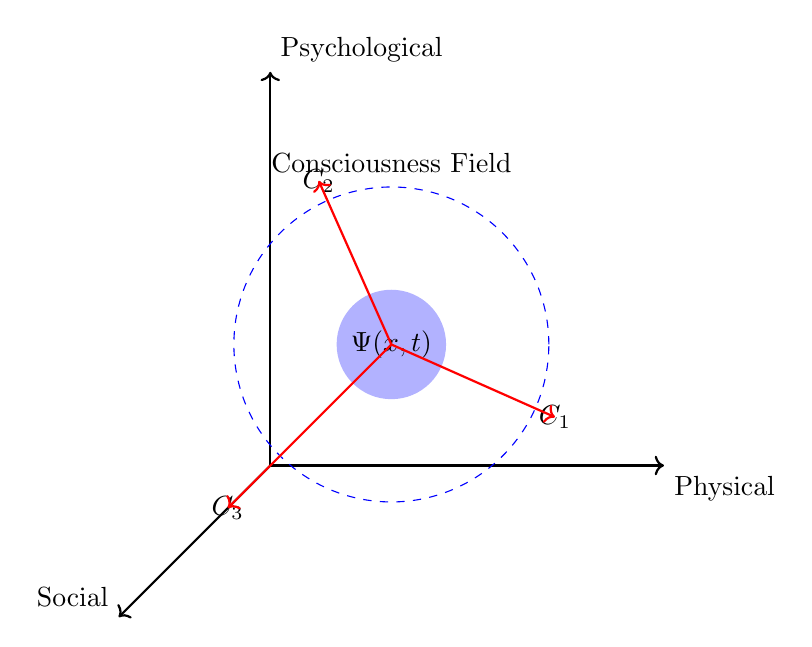
\begin{tikzpicture}
\draw[thick,->] (0,0,0) -- (5,0,0) node[anchor=north west] {Physical};
\draw[thick,->] (0,0,0) -- (0,5,0) node[anchor=south west] {Psychological};
\draw[thick,->] (0,0,0) -- (0,0,5) node[anchor=south east] {Social};
\node[circle,fill=blue!30,minimum size=1.2cm,align=center] at (2.5,2.5,2.5) {$\Psi(x,t)$};
\draw[blue,dashed] (2.5,2.5,2.5) circle (2cm);
\node[align=center] at (2.5,4.8,2.5) {Consciousness Field};
\node at (4,1,1) {$C_1$};
\node at (1,4,1) {$C_2$};
\node at (1,1,4) {$C_3$};
\draw[->,thick,red] (2.5,2.5,2.5) -- (4,1,1);
\draw[->,thick,red] (2.5,2.5,2.5) -- (1,4,1);
\draw[->,thick,red] (2.5,2.5,2.5) -- (1,1,4);
\end{tikzpicture}
\caption{Consciousness as Universal Processing Field (CUPF) model. The consciousness field $\Psi(x,t)$ penetrates physical, psychological, social, and imaginary spaces, driving decomposition and recombination.}
\label{fig:cupf}
\end{figure}

\begin{figure}[htbp]
\centering
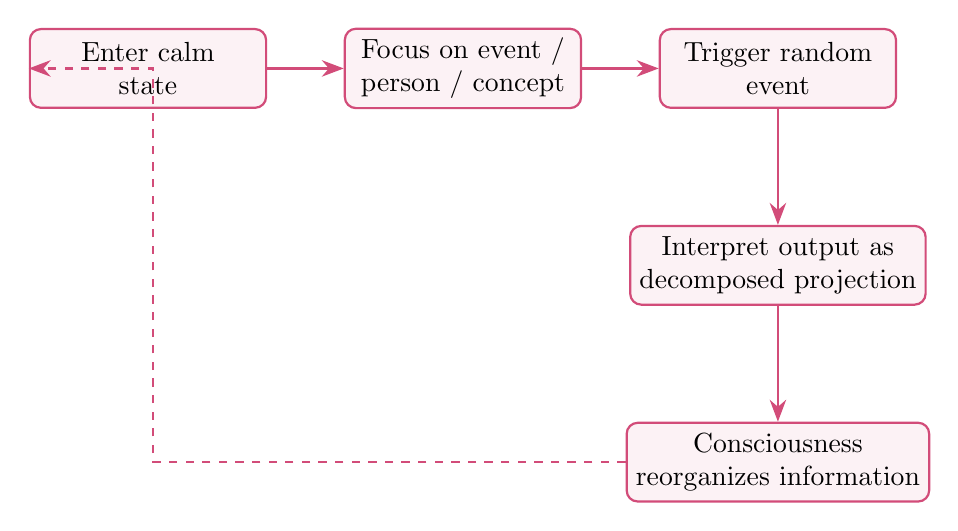
\begin{tikzpicture}[
    node distance=2cm,
    box/.style={rectangle, rounded corners, draw=purple!70, fill=purple!5, thick, minimum width=3cm, minimum height=1cm, align=center},
    arrow/.style={-{Stealth[scale=1.2]}, thick, purple!70}
]
\node[box] (calm) {Enter calm\\state};
\node[box, right of=calm, xshift=2cm] (focus) {Focus on event /\\person / concept};
\node[box, right of=focus, xshift=2cm] (trigger) {Trigger random\\event};
\node[box, below of=trigger, yshift=-0.5cm] (interpret) {Interpret output as\\decomposed projection};
\node[box, below of=interpret, yshift=-0.5cm] (reorg) {Consciousness\\reorganizes information};

\draw[arrow] (calm) -- (focus);
\draw[arrow] (focus) -- (trigger);
\draw[arrow] (trigger) -- (interpret);
\draw[arrow] (interpret) -- (reorg);
\draw[arrow, dashed] (reorg.west) -- ++(-6,0) |- (calm.west);
\end{tikzpicture}
\caption{Divination-based Decomposition Method (DDM) operational flow and information-theoretic interpretation. Random perturbation breaks the locked state, prompting consciousness to reorganize information.}
\label{fig:ddm}
\end{figure}

\end{document}
